\documentclass[11pt,a4paper]{article}

\usepackage{iftex}
\ifPDFTeX
  \usepackage[utf8]{inputenc}
  \usepackage[T1]{fontenc}
\fi
\usepackage[margin=2.2cm]{geometry}
\usepackage{amsmath,amssymb,amsthm}
\usepackage{booktabs}
\usepackage{graphicx}
\usepackage[numbers,sort&compress]{natbib}
\usepackage{xurl}
\usepackage{hyperref}
\usepackage{xcolor}
\usepackage{microtype}

\hypersetup{
  colorlinks=true,
  linkcolor=blue!60!black,
  citecolor=blue!60!black,
  urlcolor=blue!60!black
}

\emergencystretch=2em
\newcommand{\br}{\allowbreak{}}

\newtheorem{theorem}{Theorem}
\newtheorem{corollary}{Corollary}

\title{\textbf{CertMat: Formally Certified Robust Phase and Elastic Stability Verification Across One Million Inorganic Crystals}}
\author{Hyungyu Choi \\ \small Independent Researcher}
\date{November 2026}

\begin{document}
\maketitle

\begin{abstract}
Machine-learning interatomic potentials (MLIPs) and high-throughput density functional theory (DFT) workflows have expanded candidate inorganic crystal catalogs to the million-material scale, yet thermodynamic convex hull stability ($E_{\mathrm{hull}} = 0$) and mechanical Born stability ($C \succ 0$) remain evaluated almost exclusively via floating-point point estimates that neglect energy and stiffness uncertainties. Here we introduce \textbf{CertMat}, an exact rational certificate generator and machine-checked Lean~4 formal verification kernel (\texttt{leanprover/\br{}lean4:v4.16.0}, zero Mathlib dependencies, zero \texttt{sorry} or non-standard axioms across \textbf{51 mechanized theorems}) that certifies worst-case phase and elastic stability over heterogeneous uncertainty boxes. CertMat mechanizes four core theorem families: (1) exact Farkas primal-dual soundness with non-negative margin enforcement ($\delta \ge 0$) for convex hull decompositions, (2) exact algebraic cancellation of correlated elemental reference-state errors ($\sum_e c_{ie}\delta\mu_e$) proving that only uncorrelated residual errors ($\eta_i$) can flip phase stability, (3) universal worst-case interval robustness over heterogeneous energy boxes $E_i \in [L_i, U_i]$ with an exact Charnes--Cooper linear-fractional solver for the critical destabilization radius $\varepsilon^*(x)$ and adversarial decomposition \emph{Phase Switching}, and (4) exact rational $LDL^T$ Born positive-definiteness, constructive non-PD strain counterexamples, Voigt Frobenius--Weyl robustness and constructive rank-1 fragility witnesses, and bidirectional pure-rational $\mathrm{SO}(3)$-invariant Mandel/Kelvin Frobenius--Weyl robustness and constructive rank-1 fragility theorems (requiring no irrational $\sqrt{2}$). Auditing \textbf{1,044,460} unique crystal phase entries (plus \textbf{234,086} matched PBE--r2SCAN sub-hull re-audits, totaling \textbf{1,278,545} competed LP audits and 1 uncompeted elemental phase) and \textbf{34,323} valid $6\times 6$ elastic tensors across Google DeepMind GNoME (PBE and r2SCAN), NIST JARVIS-DFT 3D, and Matbench Discovery WBM---with \textbf{95,348 / 95,348} serialized TSV rational certificates machine-verified by the compiled Lean~4 \texttt{certmat-check} binary and an independent pure-\texttt{Fraction} checker (0 failures) plus 540/540 stratified spot-audit dataset-binding checks---we establish four major findings: (i) on 117,043 matched GNoME PBE-vs-r2SCAN crystals, correlated elemental shifts explain $R^2 = 73.51\%$ of formation-energy discrepancies (reducing MAE from 78.90 to 30.96~meV/atom), and CertMat's worst-case Fragile classification separates real r2SCAN stability flips with 24.65x relative risk (0.46\% vs.\ 11.36\% flip rate, ROC-AUC 0.8948) on exact 117k matched sub-hulls and 5.10x relative risk (96.40\% recall) on GNoME's primary external \texttt{Decomposition Energy Per Atom} column (6.20x relative risk / 97.46\% recall on \texttt{... MP}); (ii) \textbf{11,481 of 34,323 (33.45\%)} valid JARVIS-DFT 3D elastic tensors fail exact Born stability with Lean-certified rational strain witnesses, while \textbf{2,643 (11.57\%)} of Born-PD crystals are fragile under unconstrained 5~GPa Voigt perturbations (Lean-certified via \texttt{WEYL\_\br{}FRAGILE}) and \textbf{1,517 (6.64\%)} are fragile under $\mathrm{SO}(3)$-invariant 5~GPa Mandel perturbations (bidirectional Lean certification: 22,531 \texttt{MANDEL\_\br{}WEYL\_\br{}ROBUST} + 3,198 \texttt{MANDEL\_\br{}WEYL\_\br{}FRAGILE} witnesses); (iii) \textbf{19,894 of 42,688 (46.60\%)} WBM candidates reported stable against the static MP2020 hull collapse to strictly unstable under intra-catalog WBM competition alone (62.19\% via same-composition polymorphs, 37.81\% via cross-composition decomposition; 40.80\% even after unique-prototype deduplication); and (iv) our exact hull audit uncovered a pervasive upstream unit-scaling defect in the published NIST JARVIS-DFT 3D Figshare release (\texttt{jdft\_3d-9-24-2025.json}) consistent with dividing per-atom \texttt{optb88vdw\_\br{}total\_\br{}energy} a second time by reduced formula-unit atom count $N_{\mathrm{fu}}$, inflating \texttt{ehull > 1.0 eV/atom} for 63,386 materials (median residual 0.00677~eV vs.\ 2.605 and 2.108~eV for two negative controls).
\end{abstract}

\section{Introduction}

Automated materials discovery pipelines---exemplified by Materials Project~\cite{jain2013mp}, NIST JARVIS-DFT~\cite{choudhary2020jarvis}, WBM~\cite{wang2021wbm}, Matbench Discovery~\cite{riebesell2025matbench}, and DeepMind GNoME~\cite{merchant2023gnome}---screen hundreds of thousands of hypothetical crystals using two foundational filters: \textbf{thermodynamic phase stability} on the compositional convex hull and \textbf{mechanical Born stability} ($C \succ 0$) of the symmetrized $6\times 6$ elastic stiffness tensor~\cite{mouhat2014born}. Despite the high cost of experimental synthesis, both filters are routinely evaluated as unverified IEEE-754 floating-point point estimates:

\begin{enumerate}
  \item \textbf{Uncertainty Blindness and Chemical Heterogeneity.} Semi-local DFT (PBE/OptB88vdW) and MLIP formation energies carry systematic errors of 15--100~meV/atom whose magnitude varies nearly fivefold across chemical families (e.g., non-magnetic intermetallics vs.\ GGA+U transition-metal oxides/fluorides)~\cite{wang2021mp2020,kingsbury2022r2scan,bartel2022review}. Treating a 3~meV/atom margin identically to a 150~meV/atom margin yields substantial false-positive synthesis rates when candidates are re-evaluated at meta-GGA (r2SCAN) or experimental fidelity.
  \item \textbf{Neglected Decomposition Pathway Switching (\emph{Phase Switching}).} Under heterogeneous phase uncertainties $E_i \in [E_i - \varepsilon w_i, E_i + \varepsilon w_i]$, checking only the nominal decomposition pathway $\lambda_{\mathrm{nom}}$ is unsound: a non-nominal competing assemblage with higher nominal energy but larger uncertainty weight $w_i$ can undercut the candidate at a strictly smaller error radius $\varepsilon^*(x)$, causing naive fixed-pathway analyses to overestimate robustness by up to 52.48\%.
  \item \textbf{Numerical Fragility and Unaudited Metadata.} Floating-point convex hull solvers can misclassify near-degenerate polytopes, and upstream database metadata (\texttt{ehull}, asymmetric or crystal-symmetry-violating stiffness matrices) are rarely audited via independently checkable mathematical proofs.
\end{enumerate}

\textbf{CertMat} addresses these gaps by decoupling \emph{untrusted search} (fast HiGHS floating-point LP and numerical pre-screening) from \emph{trusted exact verification} (exact rational arithmetic over $\mathbb{Q}$, Z3 SMT exact fallback~\cite{demoura2008z3}, and a compiled Lean~4 verification kernel~\cite{demoura2021lean4}; Figure~\ref{fig:arch}).

\subsection{Related Work}
\paragraph{High-Throughput DFT Catalogs and ML Crystal Discovery.}
Large computational repositories such as the Materials Project~\cite{jain2013mp}, NIST JARVIS-DFT~\cite{choudhary2020jarvis,jarvis_figshare}, and WBM~\cite{wang2021wbm} established convex-hull stability ($E_{\mathrm{hull}}$) and mechanical stiffness screening as standard benchmarks, later scaled to millions of candidates by GNoME~\cite{merchant2023gnome} and evaluated in Matbench Discovery~\cite{riebesell2025matbench}. Prior large-scale evaluations rely almost exclusively on floating-point hull distances against static reference snapshots, leaving batch-internal hull collapse, solver degeneracy, and upstream metadata bugs largely unaudited.

\paragraph{Thermodynamic Uncertainty and Functional Transferability.}
Sun et al.~\cite{sun2016metastability} quantified the thermodynamic scale of crystalline metastability across DFT chemistries, Wang et al.~\cite{wang2021mp2020} introduced empirical GGA/GGA+U mixing correction uncertainties (MP2020), and Kingsbury et al.~\cite{kingsbury2022r2scan} benchmarked systematic PBE/SCAN-to-r2SCAN shifts. Bartel~\cite{bartel2022review} reviewed reference-state cancellation and polymorph competition in inorganic stability predictions. CertMat formalizes these physical insights into exact algebraic theorems (Theorems~2 and~3) and computes worst-case linear-fractional destabilization radii via Charnes--Cooper transformation~\cite{charnes1962fractional}.

\paragraph{Elastic Born Stability and Formal Verification.}
Mouhat and Coudert~\cite{mouhat2014born} unified necessary and sufficient Born stability conditions across crystal classes, while high-throughput repositories expose raw $6\times 6$ Voigt stiffness matrices without formal positive-definiteness or perturbation certificates. Automated SMT solvers such as Z3~\cite{demoura2008z3} and dependent-type proof assistants such as Lean~4~\cite{demoura2021lean4} are widely used in formal verification, but have seen little adoption in high-throughput materials screening.

\section{Mathematical Framework and Machine-Checked Lean~4 Kernel}

All four core theorem families and executable certificate checkers are formalized in pure Lean~4 (\texttt{leanprover/lean4:v4.16.0}) with zero external Mathlib dependencies across \texttt{lean/\br{}CertMat/\br{}\{ExactRat,\br{}Farkas,\br{}RefErrorCancel,\br{}IntervalHull,\br{}BornElastic,\br{}Checker\}.lean} and \texttt{lean/\br{}Main.lean}. Static scanning (blocking \texttt{sorry}, \texttt{axiom}, \texttt{admit}, \texttt{implemented\_\br{}by}, \texttt{extern}, \texttt{unsafe}, \texttt{partial}, \texttt{opaque}, \texttt{native\_\br{}decide}, \texttt{csimp}) and mechanical \texttt{\#print axioms} auditing confirm that all \textbf{51 core theorems} depend solely on Lean's standard logical axioms (\texttt{propext}, \texttt{Classical.choice}, \texttt{Quot.sound}) with \textbf{0 \texttt{sorryAx}}.

\subsection{Theorem 1: Farkas Primal-Dual Soundness for Phase Stability}
Let $c_i \in \mathbb{Q}_{\ge 0}^E$ ($i = 1,\dots,m$) and $c_x \in \mathbb{Q}_{\ge 0}^E$ be normalized atomic compositions ($\sum_e c_{ie} = \sum_e c_{xe} = 1$, verified inside Lean by \texttt{checkNormalizedComps}) with per-atom energies $E_i, E_x \in \mathbb{Q}$. A composition-conserving decomposition $\lambda \in \mathbb{Q}_{\ge 0}^m$ satisfies $\sum_{i=1}^m \lambda_i c_{ie} = c_{xe}$ for all $e$, implying $\sum_i \lambda_i = 1$ (\texttt{valid\_\br{}decomp\_\br{}sum\_\br{}one}).

\begin{theorem}[Primal Instability and Dual Stability]
(a) A valid decomposition $\lambda$ with $\sum_i \lambda_i E_i < E_x$ certifies unconditional instability and rules out any dual certificate $\mu$ with margin $\delta \ge 0$ (\texttt{farkas\_\br{}primal\_\br{}unstable\_\br{}excludes\_\br{}dual}).
(b) A chemical potential $\mu \in \mathbb{Q}^E$ satisfying $\delta \ge 0$, $\mu \cdot c_i \le E_i$ ($\forall i$), and $E_x + \delta \le \mu \cdot c_x$ certifies $\sum_i \lambda_i E_i \ge E_x + \delta \ge E_x$ for every valid decomposition $\lambda$ (\texttt{farkas\_\br{}dual\_\br{}stable\_\br{}sound}, \texttt{checkDualStable\_\br{}on\_\br{}hull\_\br{}sound}). Enforcing \texttt{ble 0 delta} in \texttt{checkDualStable} blocks negative-margin spoofing.
(c) Simultaneous attainment of $(\mu,\delta)$ and $\lambda^*$ with $\sum_i \lambda^*_i E_i = E_x + \delta$ uniquely determines the exact convex hull margin (\texttt{farkas\_\br{}exact\_\br{}margin\_\br{}unique}).
\end{theorem}

\subsection{Theorem 2: Exact Cancellation of Correlated Elemental Reference Errors}
Modeling true formation energies as $E_i^{\mathrm{true}} = E_i + \sum_{e=1}^E c_{ie}\delta\mu_e + \eta_i$ and $E_x^{\mathrm{true}} = E_x + \sum_{e=1}^E c_{xe}\delta\mu_e + \eta_x$:

\begin{theorem}[Elemental-Shift Cancellation and Dual Invariance]
For every valid decomposition $\lambda$,
\begin{equation}
  E_x^{\mathrm{true}} - \sum_{i=1}^m \lambda_i E_i^{\mathrm{true}}
  = \left(E_x - \sum_{i=1}^m \lambda_i E_i\right) + \left(\eta_x - \sum_{i=1}^m \lambda_i \eta_i\right),
\end{equation}
so correlated elemental shifts $\delta\mu$ cancel identically to zero (\texttt{ref\_\br{}error\_\br{}exact\_\br{}cancellation}). When $\eta = 0$, shifting $\mu' = \mu + \delta\mu$ preserves the exact stability margin $\delta$ for arbitrarily large $\delta\mu$ (\texttt{only\_\br{}residual\_\br{}error\_\br{}flips\_\br{}stability}).
\end{theorem}

\subsection{Theorem 3: Heterogeneous Interval Robustness, Exact $\varepsilon^*(x)$, and Phase Switching}
Over a heterogeneous uncertainty hyperbox $E_i^{\mathrm{true}} \in [L_i, U_i]$, $E_x^{\mathrm{true}} \in [L_x, U_x]$ constructed inside the Lean TCB from $(E_i, E_x)$, non-negative weights $(w_i, w_x)$, and radius $\varepsilon \ge 0$ ($L_i = E_i - \varepsilon w_i$, $U_i = E_i + \varepsilon w_i$):

\begin{theorem}[Worst-Case Corner Universality and Critical Radius]
A single dual certificate $\mu$ at $(U_x, L)$ with $\delta \ge 0$ certifies universal stability across the entire continuous hyperbox (\texttt{interval\_\br{}robust\_\br{}stable\_\br{}universal}); a single primal witness $\lambda$ at $(L_x, U)$ certifies universal instability across the entire hyperbox (\texttt{interval\_\br{}robust\_\br{}unstable\_\br{}universal}). For $w_i, w_x \ge 0$, the exact signed critical flip radius is
\begin{equation}
  r^*(x) = \min_{\lambda \in \Lambda(x)} \frac{\sum_{i=1}^m \lambda_i E_i - E_x}{w_x + \sum_{i=1}^m \lambda_i w_i}, \qquad \varepsilon^*(x) = |r^*(x)|,
\end{equation}
computed exactly via the Charnes--Cooper transformation~\cite{charnes1962fractional} $t = (w_x + \sum_i \lambda_i w_i)^{-1} > 0$, $y_i = t\lambda_i$:
\begin{equation}
  \min_{y \ge 0,\; t \ge 0} \sum_{i=1}^m E_i y_i - E_x t \quad \mathrm{s.t.} \quad \sum_{i=1}^m c_{ie} y_i - c_{xe} t = 0\;(\forall e), \quad \sum_{i=1}^m w_i y_i + w_x t = 1.
\end{equation}
\end{theorem}

Because $\sum_e c_{ie} = 1$, $t=0$ forces $y=0$, violating the weight normalization constraint; hence $t > 0$ holds automatically. Zero-weight strictly unstable pathways yield $r^* = -\infty$, whereas zero-weight ties ($E^T\lambda = E_x$ with denominator $0$) cannot strictly destabilize $x$ under the non-strict $\le$ convention and do not mask positive-denominator pathways (yielding $r^* = +\infty$ when no positive-weight pathway exists). Constructive \texttt{INTERVAL\_\br{}FRAGILE\_\br{}DESTAB} and \texttt{INTERVAL\_\br{}FRAGILE\_\br{}STAB} certificates witness concrete in-box realizations that flip stability. Whenever an adversarial assemblage $\lambda_{\mathrm{adv}}$ achieves a strictly smaller critical scale than a nominal decomposition $\lambda_{\mathrm{nom}}$, \emph{Phase Switching} occurs.

\subsection{Theorem 4: Exact Rational Born Stability, Voigt/Mandel Weyl Robustness, and Fragility}
Let $C \in \mathbb{Q}^{6\times 6}$ be the symmetrized Voigt stiffness tensor $C_{\mathrm{sym}} = \frac{1}{2}(C + C^T)$.

\begin{theorem}[Exact Rational $LDL^T$ and Bidirectional Pure-Rational Mandel Weyl Bounds]
(a) Exact rational $C = L\operatorname{diag}(d)L^T$ ($L$ unit lower-triangular, $d_k > 0$) certifies $v^T C v > 0$ for all $v \ne 0$ (\texttt{born\_\br{}pd\_\br{}of\_\br{}ldlt}); conversely, any $d_k \le 0$ constructs an exact nonzero strain counterexample $v \in \mathbb{Q}^6$ via back-substitution satisfying $v^T C v = d_k \le 0$ (\texttt{not\_\br{}born\_\br{}pd\_\br{}of\_\br{}witness}).
(b) In Voigt norm, shifted $LDL^T$ on $C - \lambda_0 I$ with $0 \le \delta \le \lambda_0$ certifies $C + \Delta C \succ 0$ for all $\|\Delta C\|_F \le \delta$ (\texttt{shifted\_\br{}ldlt\_\br{}frob\_\br{}robust\_\br{}born}); conversely, \texttt{WEYL\_\br{}FRAGILE} witnesses ($v \ne 0$, $v^T C v \le \delta \|v\|_2^2$) synthesize $\Delta C = -\delta (vv^T / \|v\|_2^2)$ with $\|\Delta C\|_F = \delta$ breaking Born stability (\texttt{weyl\_\br{}fragile\_\br{}of\_\br{}witness}).
(c) Using reciprocal rational weights $s = (1,1,1,1/2,1/2,1/2)$ and $r = (1,1,1,2,2,2)$ ($s_i r_i = 1$) without irrational $\sqrt{2}$, a shifted $LDL^T$ certificate on $C_{\mathrm{Voigt}} - \lambda_0 \operatorname{diag}(s)$ certifies $C + \Delta C \succ 0$ for every perturbation satisfying the squared $\mathrm{SO}(3)$-invariant Mandel Frobenius norm bound $\|D\Delta C D\|_F^2 = \sum_{i,j} r_i r_j (\Delta C_{ij})^2 \le \delta^2$ ($0 \le \delta \le \lambda_0$; \texttt{weighted\_\br{}shifted\_\br{}ldlt\_\br{}frob\_\br{}robust\_\br{}born}, \texttt{checkMandelWeylRobustBorn\_\br{}frob\_\br{}sound}). Conversely, a \texttt{MANDEL\_\br{}WEYL\_\br{}FRAGILE} witness ($v \ne 0$, $v^T C v \le \delta \|v\|_s^2$) constructively synthesizes $\Delta C_{ij} = -(\delta / \|v\|_s^2)(s_i v_i)(s_j v_j)$ satisfying exact $\|D\Delta C D\|_F^2 = \delta^2$ and $v^T(C + \Delta C)v \le 0$ (\texttt{weighted\_\br{}weyl\_\br{}fragile\_\br{}of\_\br{}witness}, \texttt{checkMandelWeylFragile\_\br{}sound}).
\end{theorem}

\subsection{Hybrid Exact Solver Architecture}
\texttt{certmat/exact\_lp.py} pairs a HiGHS active-basis recovery path (reconstructing exact \texttt{Fraction} primal/dual solutions via Gauss--Jordan elimination with zero-tolerance verification) with an exact Z3 SMT/Optimize fallback~\cite{demoura2008z3} for degenerate polytopes (1.37\% of all LP audits; Figure~\ref{fig:arch}).

\begin{figure}[t]
  \centering
  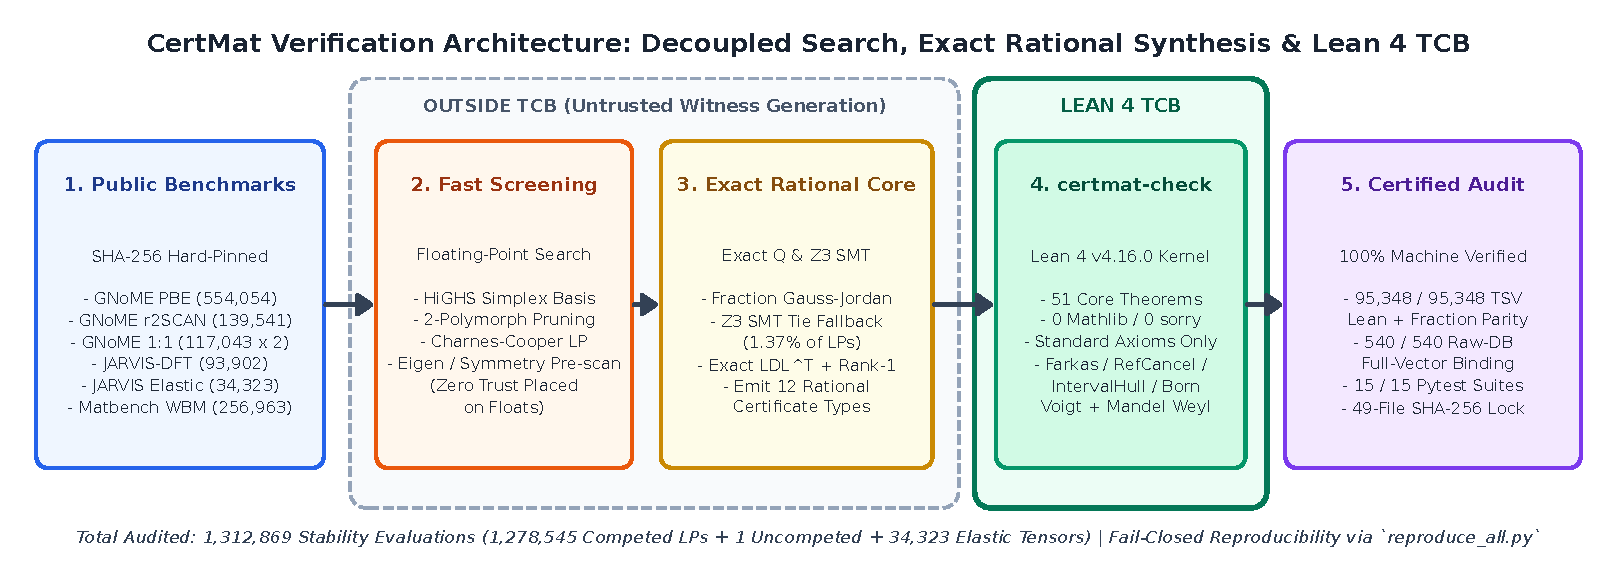
\includegraphics[width=\textwidth]{figures/fig5_certmat_architecture.pdf}
  \caption{CertMat architecture separating untrusted floating-point search (HiGHS LP and numerical pre-screening) from exact rational witness synthesis (\texttt{Fraction} + Z3 SMT fallback) and the self-contained Lean~4 v4.16.0 Trusted Computing Base (\texttt{certmat-check}, 51 mechanized theorems, 0 \texttt{sorry}).}
  \label{fig:arch}
\end{figure}

\section{Experimental Setup, Datasets, and Verification Scope}

We audited four public benchmark databases with source-code-pinned SHA-256 checksums (\texttt{PINNED\_\br{}DATASET\_\br{}SHA256} in \texttt{certmat/\br{}datasets.py} and \texttt{data/\br{}dataset\_\br{}manifest.json}): Table~\ref{tab:datasets}.

\begin{table}[h]
\centering
\caption{Audited public materials databases, Z3 fallback rates, and compiled Lean~4 TSV verification totals.}
\label{tab:datasets}
\resizebox{\textwidth}{!}{%
\begin{tabular}{@{}llrrr@{}}
\toprule
Dataset & Scope & Audited & Z3 Fallback & Lean~4 Verified \\
\midrule
NIST JARVIS-DFT 3D~\cite{choudhary2020jarvis,jarvis_figshare} & Self-contained OptB88vdW hull & 93,902 (+1 uncomp.) & 864 (0.92\%) & 5,000 / 5,000 \\
NIST JARVIS-DFT 3D Elastic & Valid $6\times 6$ tensors (179 skipped) & 34,323 & N/A ($LDL^T$) & 39,619 Voigt + 25,729 Mandel \\
Matbench Discovery WBM~\cite{wang2021wbm,riebesell2025matbench} & Intra-catalog MP2020 hull & 256,963 & 3,271 (1.27\%) & 5,000 / 5,000 \\
GNoME PBE Full~\cite{merchant2023gnome} & Intra-catalog + MP/OQMD margins & 554,054 & 13,090 (2.36\%) & 5,000 / 5,000 \\
GNoME r2SCAN Full~\cite{merchant2023gnome} & Intra-catalog r2SCAN hull & 139,541 & 116 (0.08\%) & 5,000 / 5,000 \\
GNoME Matched PBE--r2SCAN & Exact 1:1 sub-hull (117,043 $\times$ 2) & 234,086 & 129 (0.06\%) & 5,000 PBE + 5,000 r2SCAN \\
\midrule
\textbf{Total} & \textbf{4 Public Materials Databases} & \textbf{1,312,869} & \textbf{17,470 (1.37\% LP)} & \textbf{95,348 / 95,348 (100.0\%)} \\
\bottomrule
\end{tabular}%
}
\end{table}

We evaluate uniform radii $\varepsilon \in \{10, 25, 50\}$~meV/atom, a literature-motivated chemistry profile (\texttt{HETERO\_\br{}CHEM\_\br{}PROFILE}: 10~meV elemental reference, 15~meV intermetallic, 25~meV chalcogenide/pnictide, 30~meV main-group halide/oxide, 35~meV GGA+U non-oxide, 45~meV f-block non-oxide, 50~meV GGA+U oxide/fluoride, 55~meV f-block oxide/fluoride), a zero-elemental-reference ablation ($\sigma_{\mathrm{elem}} = 0$), and 5-fold out-of-sample Theorem~2 residual calibration.

\section{Results}

\subsection{Empirical Verification of Theorem 2 and GNoME PBE-vs-r2SCAN Cross-Validation}
Across all \textbf{117,043} matched GNoME crystals with both PBE and r2SCAN formation energies, orthogonal least-squares decomposition $\Delta E_f(\mathrm{r2SCAN}-\mathrm{PBE}) = \sum_e c_{ie}\delta\mu_e + \eta_i$ (full rank 83, condition number 697.3) empirically validates Theorem~2: raw MAE drops from \textbf{78.90~meV/atom} (RMSE 101.03~meV/atom) to residual MAE \textbf{30.96~meV/atom} (\textbf{60.76\% reduction}, RMSE 50.65~meV/atom), with correlated elemental shifts explaining $R^2 = 73.51\%$ of variance. Irreducible residual MAE spans a \textbf{4.75x} chemical spread from \texttt{intermetallic} (19.93~meV/atom, 7.16\% flip rate, 0.30\% $>25$~meV flip rate) to \texttt{ggau\_\br{}oxide\_\br{}fluoride} (94.65~meV/atom, 39.09\% flip rate, 18.28\% $>25$~meV flip rate; 60x severe-flip disparity; Table~\ref{tab:gnome_cls} and Figure~\ref{fig:gnome}).

\begin{table}[h]
\centering
\caption{Matched GNoME PBE-to-r2SCAN Theorem~2 residual errors, OOS literature-box coverage ($|\eta| \le w$), and actual r2SCAN flip rates ($N=116,988$ external PBE-stable phases).}
\label{tab:gnome_cls}
\resizebox{\textwidth}{!}{%
\begin{tabular}{@{}lrrrrrr@{}}
\toprule
Chemistry Class & $N$ & $\eta$ MAE (meV) & p75 (meV) & Lit-Box Cov. & Flip ($>0$) & Severe ($>25$ meV) \\
\midrule
\texttt{intermetallic} & 12,157 & 19.93 & 26.37 & 46.22\% & 7.16\% & 0.30\% \\
\texttt{chalcogenide\_pnictide} & 7,059 & 28.38 & 38.13 & 58.58\% & 7.28\% & 0.86\% \\
\texttt{f\_block\_non\_oxide} & 70,913 & 24.86 & 32.00 & 85.34\% & 11.64\% & 2.60\% \\
\texttt{halide\_oxide\_main} & 4,821 & 65.38 & 98.58 & 33.29\% & 16.08\% & 3.82\% \\
\texttt{f\_block\_oxide\_fluoride} & 6,658 & 67.86 & 92.88 & 55.48\% & 17.23\% & 4.96\% \\
\texttt{tm\_non\_oxide} & 13,236 & 33.73 & 43.67 & 67.91\% & 24.36\% & 10.16\% \\
\texttt{ggau\_oxide\_fluoride} & 2,144 & 94.65 & 132.13 & 35.07\% & \textbf{39.09\%} & \textbf{18.28\%} \\
\midrule
\textbf{All Matched (Ext.\ MP-Ref)} & \textbf{116,988} & \textbf{30.96} & --- & \textbf{72.92\%} & \textbf{13.35\%} & \textbf{3.58\%} \\
\bottomrule
\end{tabular}%
}
\end{table}

On the 1:1 matched 117k exact Charnes--Cooper LP sub-hull ($N=116,877$ PBE-stable phases, 5,231 flips, 0 monotonicity violations vs.\ \texttt{Decomposition Energy Per Atom All}), the heterogeneous profile separates flips with \textbf{24.65x relative risk} (0.46\% vs.\ 11.36\%, 93.50\% recall, ROC-AUC 0.8948; uniform 25~meV achieves 22.84x and ROC-AUC 0.8969). On the 10k-phase chemical-system GroupKFold exact LP (transductive fixed-catalog hull), OOS empirical-MAE calibration achieves \textbf{31.59x} relative risk (0.41\% vs.\ 12.90%), with modest non-significant $\Delta\mathrm{AUC} = +0.0017$ (cluster-bootstrap 95\% CI $[-0.0002, +0.0037]$; $\sigma_{\mathrm{elem}}=0$ ablation: 27.79x, AUC 0.8966). On the external \texttt{Decomposition Energy Per Atom} proxy ($N=116,988$), literature heterogeneous boxes achieve \textbf{5.10x} relative risk (96.40\% recall; 6.20x / 97.46\% on \texttt{... MP}), and GroupKFold OOS residual calibration significantly improves ranking AUC over uniform proxies from 0.7061 to \textbf{0.7242} ($\Delta = +0.0180$, CI $[+0.0162, +0.0200]$) for $>0$ flips and 0.5959 to \textbf{0.6402} ($\Delta = +0.0443$, CI $[+0.0404, +0.0482]$) for $>25$~meV severe flips (supervised logistic regression baseline using flip labels: 0.7388 / 0.7270).

On full \textbf{GNoME PBE (554,054)} and \textbf{GNoME r2SCAN (139,541)}, median official external stability margin is 24.0~meV/atom (25~meV proxy fragility 77.38\%; 80.34\% on \texttt{... MP}; 88.68\% on \texttt{... MP OQMD}). Internally, \textbf{12,461 / 416,084 (2.99\%)} PBE and \textbf{4,552 / 131,784 (3.45\%)} r2SCAN nominally stable phases exhibit \emph{Phase Switching} (59 and 27 critical reversals; max overestimation 34.48\% in \texttt{a403464fde} $\mathrm{Gd}_2\mathrm{Ru}_4\mathrm{Y}_{10}$ and 50.52\% in \texttt{32d32e7908} $\mathrm{C}_2\mathrm{CeFe}_2$).

\begin{figure}[t]
  \centering
  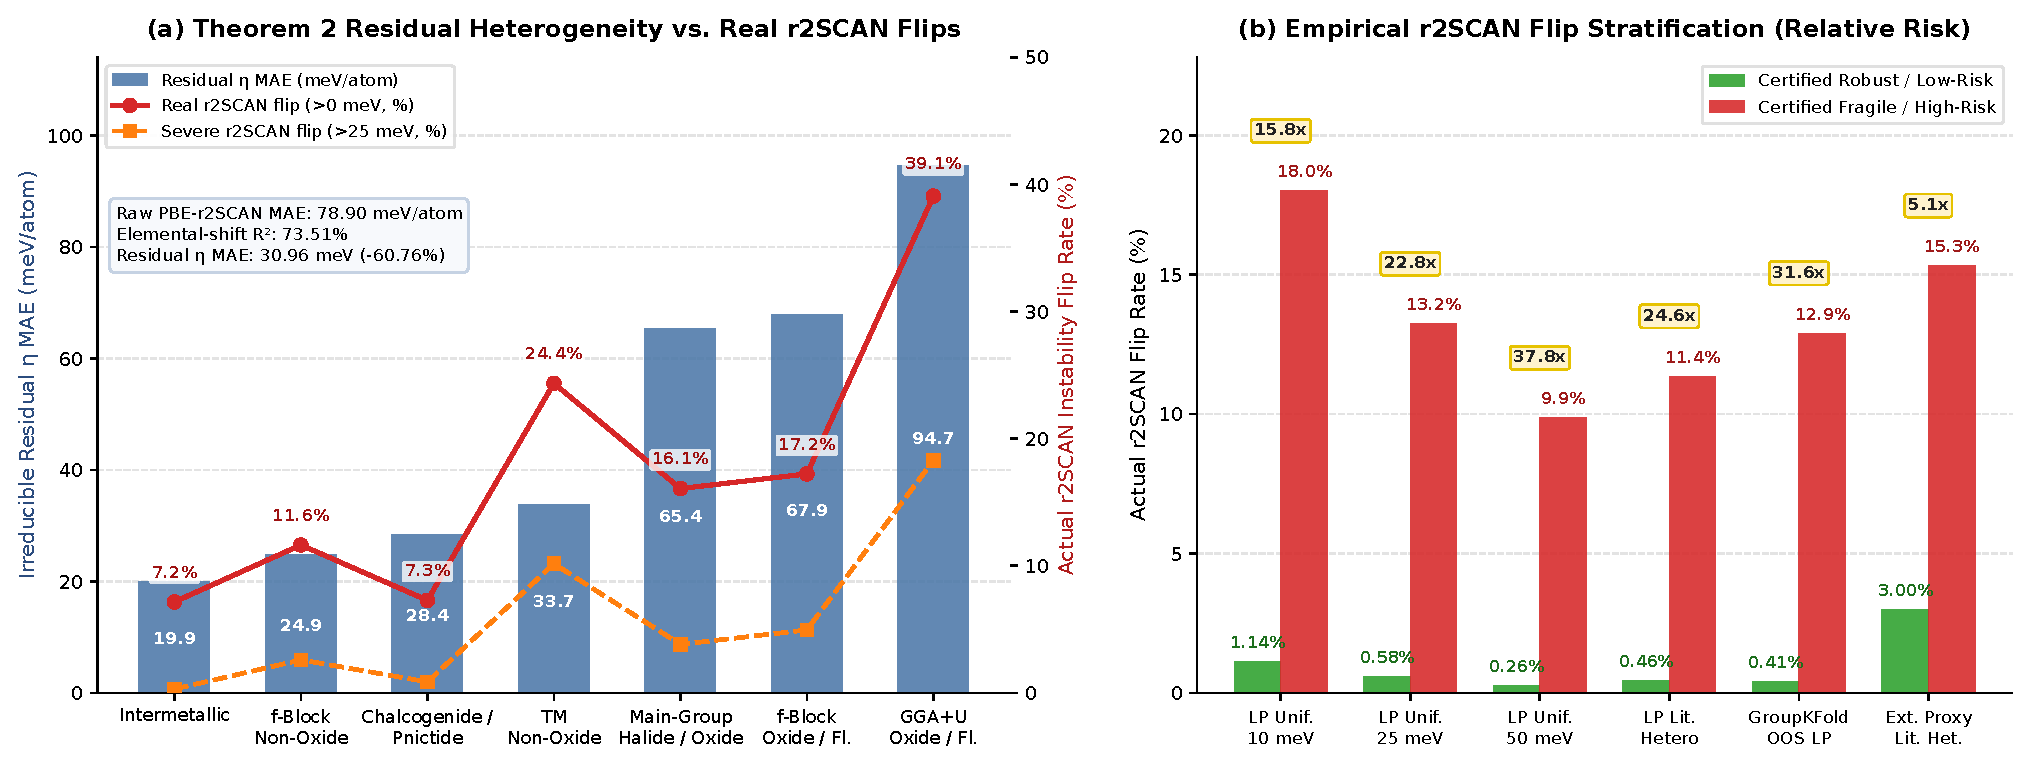
\includegraphics[width=\textwidth]{figures/fig1_gnome_theorem2_and_crossval.pdf}
  \caption{(a) Theorem~2 orthogonal decomposition across 117,043 matched GNoME PBE-vs-r2SCAN crystals: correlated elemental shifts explain $R^2 = 73.51\%$ of discrepancy variance, while residual MAE $\eta$ spans a 4.75x chemical-class spread matching actual r2SCAN flip rates. (b) Empirical r2SCAN instability stratification across exact LP and external proxy regimes.}
  \label{fig:gnome}
\end{figure}

\subsection{NIST JARVIS-DFT 3D Phase Audit \& Discovery of Upstream \texttt{ehull} Corruption}
Auditing all \textbf{93,902} JARVIS-DFT 3D entries on their exact self-contained OptB88vdW hull (93,901 competed + 1 uncompeted elemental phase) yields \textbf{25,908} nominally stable and \textbf{67,993} unstable phases (14,185 same-composition polymorphs, 53,808 cross-composition). Among ground states, \textbf{44.28\%} (11,473) are fragile at 10~meV/atom, \textbf{69.76\%} (18,074) at 25~meV/atom, \textbf{86.76\%} (22,479) at 50~meV/atom, and \textbf{76.06\%} (19,706) under the heterogeneous profile (\textbf{75.36\%} / 19,524 under $\sigma_{\mathrm{elem}}=0$ ablation, where Phase Switching rises from 921 [3.55\%] to 1,232 [4.76\%]). Maximum Phase Switching overestimation reaches \textbf{52.48\%} in \texttt{JVASP-14649} ($\mathrm{NpCo}_2$), with 17 critical reversals. Raw \texttt{optb88vdw\_\br{}total\_\br{}energy} and \texttt{formation\_\br{}energy\_\br{}peratom} hulls agree to \textbf{0.005~meV/atom} median on 1,000 stratified phases ($R^2 = 0.999941$).

Crucially, comparing our exact hull against the published \texttt{ehull} field in the Figshare release (\texttt{jdft\_3d-9-24-2025.json}~\cite{jarvis_figshare}, SHA-256 \texttt{9dacb55ac8371c...}) uncovered an unreported upstream unit-scaling defect: \textbf{63,386} of 93,902 entries have \texttt{ehull > 1.0 eV/atom} (median \textbf{1.7189~eV/atom}), including \textbf{16,898 (65.22\%)} of CertMat's 25,908 ground states. Across \textbf{92,955} multinary entries, dividing per-atom \texttt{optb88vdw\_\br{}total\_\br{}energy} a second time by formula-unit atom count $N_{\mathrm{fu}}$ ($(E_{\mathrm{optB88}}/N_{\mathrm{fu}}) - E_{\mathrm{elem\_hull}}$) reproduces published \texttt{ehull} with median absolute residual \textbf{0.00677~eV/atom} (\textbf{66.69\%} within 0.01~eV; \textbf{84.72\%} within 0.05~eV), versus \textbf{2.6047~eV} (0.95\% match) and \textbf{2.1078~eV} (1.20\% match) for two negative controls (Figure~\ref{fig:jarvis_bug}; standalone reproduction script in \texttt{scripts/\br{}repro\_\br{}jarvis\_\br{}ehull\_\br{}bug.py} and draft issue in \texttt{paper/\br{}jarvis\_\br{}issue\_\br{}draft.md}). Algorithmically selected zero-residual ground states include \texttt{JVASP-106708} ($\mathrm{U}_2\mathrm{Pd}_3\mathrm{Rh}_3$, $N_{\mathrm{fu}}=8$, published \texttt{3.6460~eV}), \texttt{JVASP-15157} ($\mathrm{TbB}_2\mathrm{Ru}_3$, $N_{\mathrm{fu}}=6$, \texttt{4.3407~eV}), \texttt{JVASP-13318} ($\mathrm{BaNd}_2\mathrm{Se}_4$, $N_{\mathrm{fu}}=7$, \texttt{1.1113~eV}), and \texttt{JVASP-152492} ($\mathrm{TbAlPt}$, $N_{\mathrm{fu}}=3$, \texttt{1.2969~eV}), whereas single-element entries ($N_{\mathrm{fu}}=1$, 915 phases) are unaffected (median \texttt{0.0317~eV/atom}).

\begin{figure}[t]
  \centering
  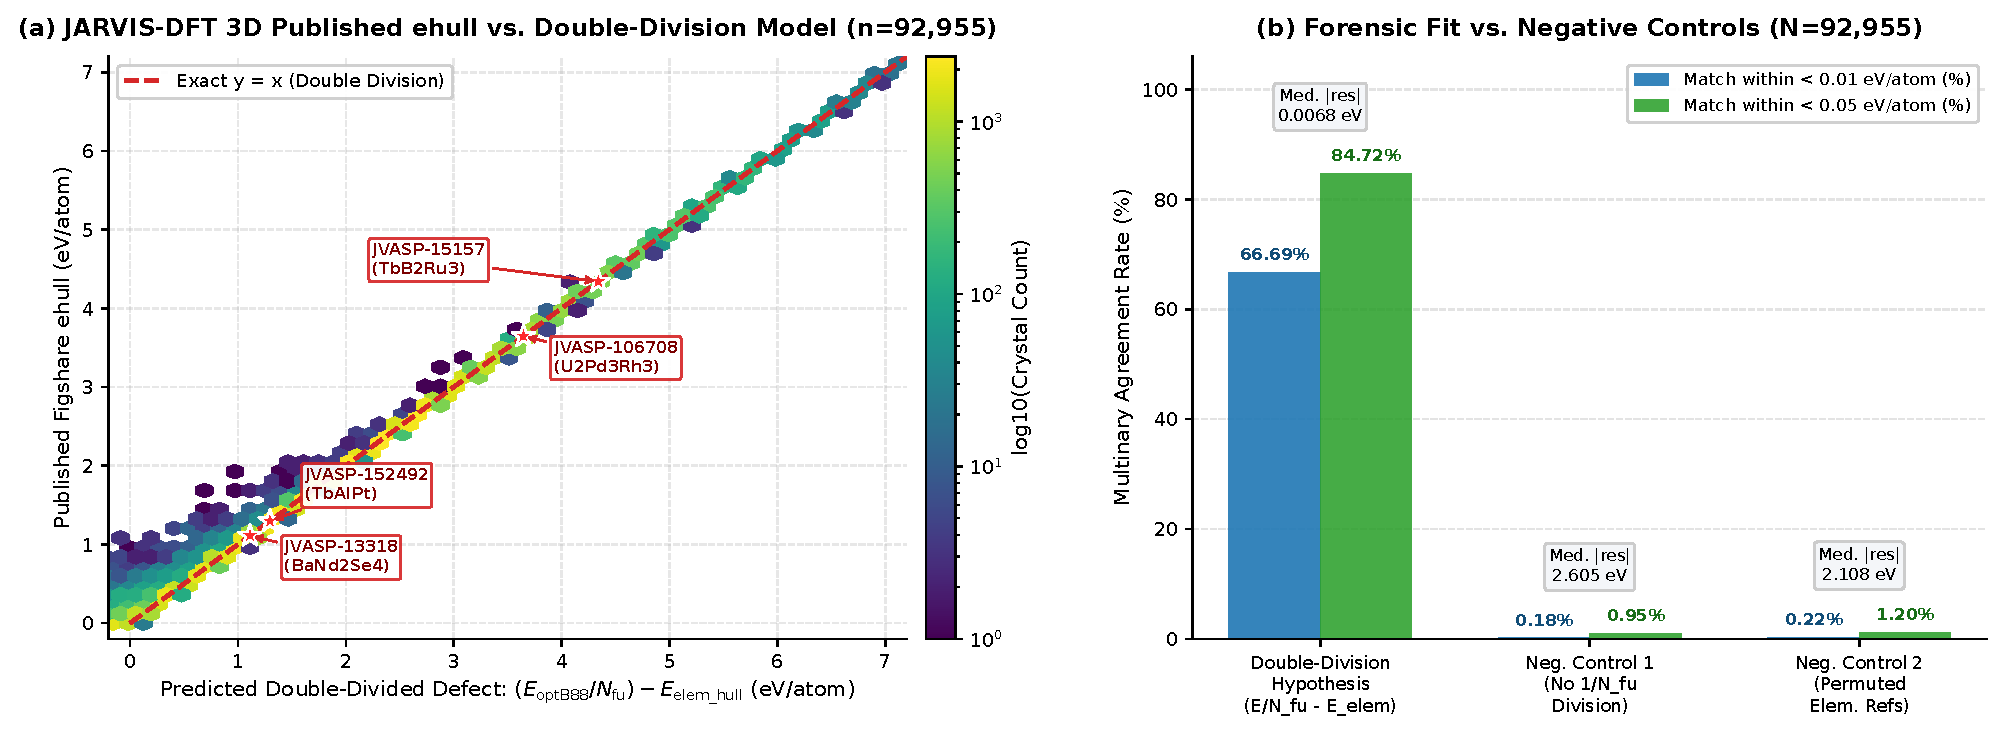
\includegraphics[width=\textwidth]{figures/fig2_jarvis_ehull_forensic.pdf}
  \caption{(a) Log-density hexbin comparison between predicted double-divided $(E_{\mathrm{optB88}}/N_{\mathrm{fu}}) - E_{\mathrm{elem\_hull}}$ and published \texttt{ehull} across 92,955 multinary JARVIS entries, highlighting exact zero-residual stable ground states. (b) Agreement rates against two negative controls.}
  \label{fig:jarvis_bug}
\end{figure}

\subsection{Matbench Discovery WBM (256,963 Crystals): Batch Hull Collapse}
Across all \textbf{256,963} WBM entries (215,488 unique prototypes), \textbf{44,667} are nominally stable on the intra-catalog MP2020-corrected hull (\textbf{73.51\%} fragile at 25~meV; \textbf{79.81\%} under heterogeneous boxes; \textbf{1,439 / 3.22\%} Phase Switching, max overestimation 35.51\% in \texttt{wbm-2-50242}). Among the \textbf{42,688} candidates labeled stable against the \emph{static} MP2020 hull, \textbf{19,894 (46.60\%)} collapse to strictly unstable under intra-WBM competition alone: \textbf{12,372 (62.19\%)} via same-composition polymorphs and \textbf{7,522 (37.81\%)} via cross-composition decomposition (\textbf{13,385 / 32,805 = 40.80\%} even after prototype deduplication; Figure~\ref{fig:wbm}). Elemental linear shifts explain $R^2 = 85.04\%$ of MP2020 corrections (MAE 108.22 to 29.62~meV/atom), leaving 279.99~meV/atom residual MAE in \texttt{ggau\_\br{}oxide\_\br{}fluoride}.

\begin{figure}[t]
  \centering
  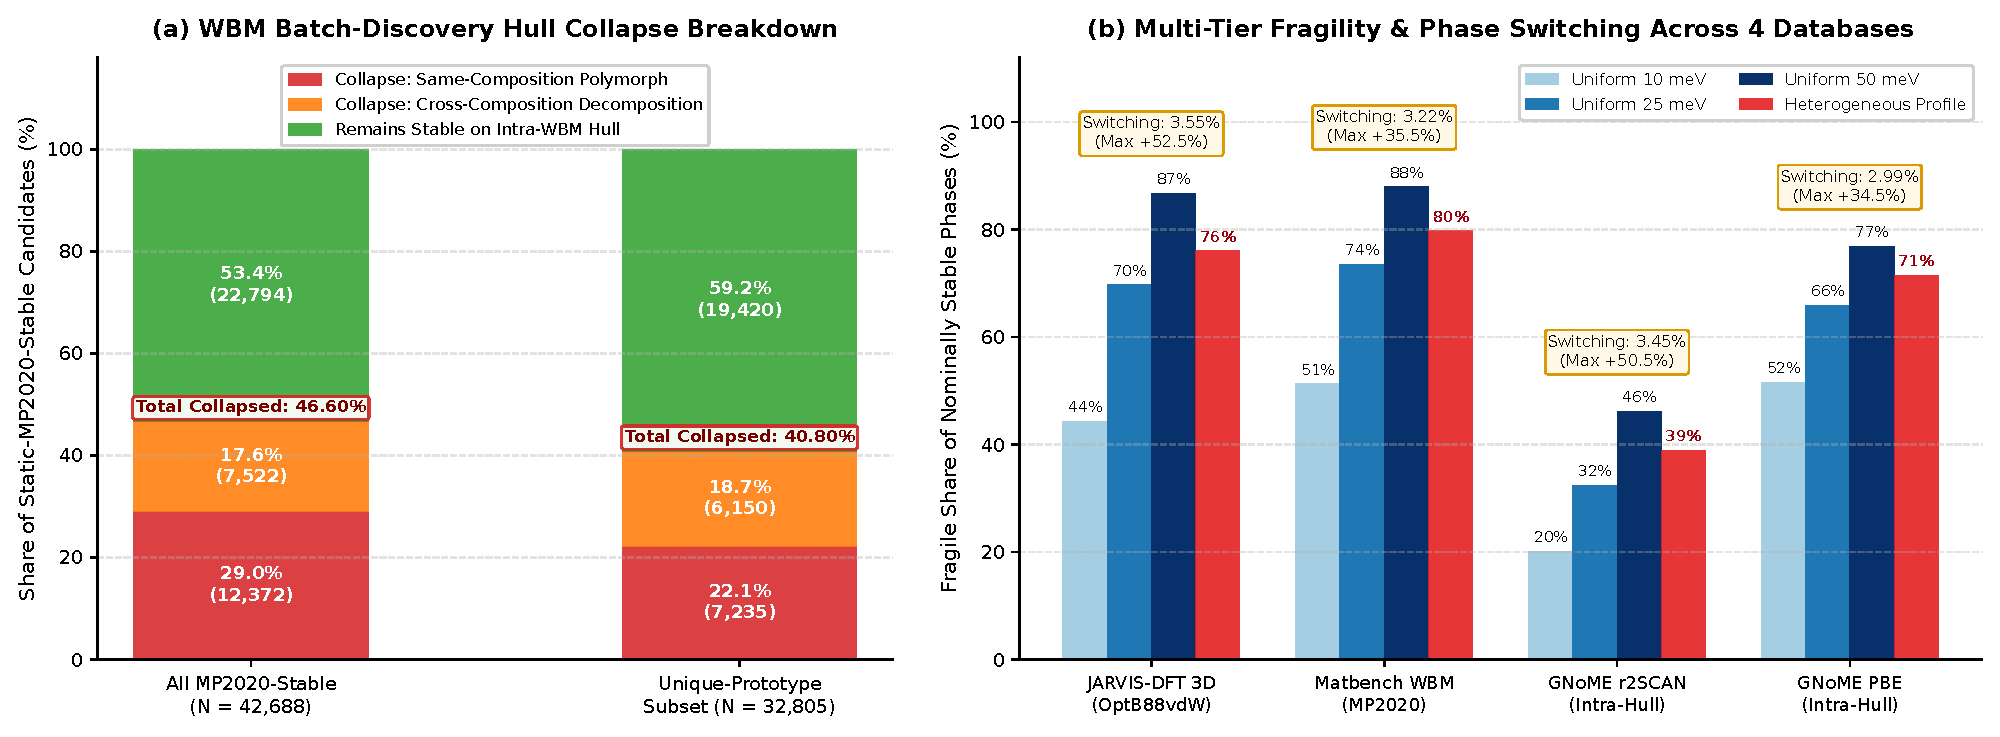
\includegraphics[width=\textwidth]{figures/fig4_wbm_collapse_and_phase_switching.pdf}
  \caption{(a) Intra-catalog collapse breakdown of 42,688 WBM candidates reported stable against the static MP2020 hull (and 32,805 after unique-prototype deduplication) into same-composition polymorphs vs.\ cross-composition decompositions. (b) Multi-tier fragility and heterogeneous Phase Switching across all four audited phase databases.}
  \label{fig:wbm}
\end{figure}

\subsection{NIST JARVIS-DFT 3D $6\times 6$ Elastic Tensor Audit (34,323 Crystals)}
Auditing all \textbf{34,323} valid $6\times 6$ stiffness tensors in \texttt{jdft\_3d.json} (179 malformed skipped) yields \textbf{22,842 (66.55\%)} Born-PD and \textbf{11,481 (33.45\%)} Born non-PD crystals (3,712 mild $[-10,0]$, 3,960 moderate $[-50,-10)$, 3,542 severe $[-1000,-50)$, 267 numerical blow-ups $<-1000$~GPa), all with \textbf{65,348 / 65,348} Lean~4 certificates verified (39,619 Voigt + 25,729 Mandel: \textbf{22,531} \texttt{MANDEL\_\br{}WEYL\_\br{}ROBUST} + \textbf{3,198} \texttt{MANDEL\_\br{}WEYL\_\br{}FRAGILE}; Figure~\ref{fig:elastic}). Under 1/5/10~GPa perturbations, \textbf{311 (1.36\%) / 1,517 (6.64\%) / 3,198 (14.00\%)} of Born-PD crystals are fragile in the $\mathrm{SO}(3)$-invariant Mandel metric, compared with \textbf{490 (2.15\%) / 2,643 (11.57\%) / 5,296 (23.19\%)} under unconstrained Voigt perturbations. Under VASP OUTCAR shear ordering, \textbf{598 (1.74\%)} violate matrix symmetry ($>1$~GPa, 0 in PD), \textbf{2,805 (8.17\%)} violate crystal-system symmetry allowing axis permutations (401 / 1.76\% in PD; 5,606 / 2,358 under fixed standard axes), and \textbf{1,442 / 9,096 (15.85\%)} cubics violate coordinate-free Mandel eigenvalue multiplicity (205 / 6,232 = 3.29\% in PD).

\begin{figure}[t]
  \centering
  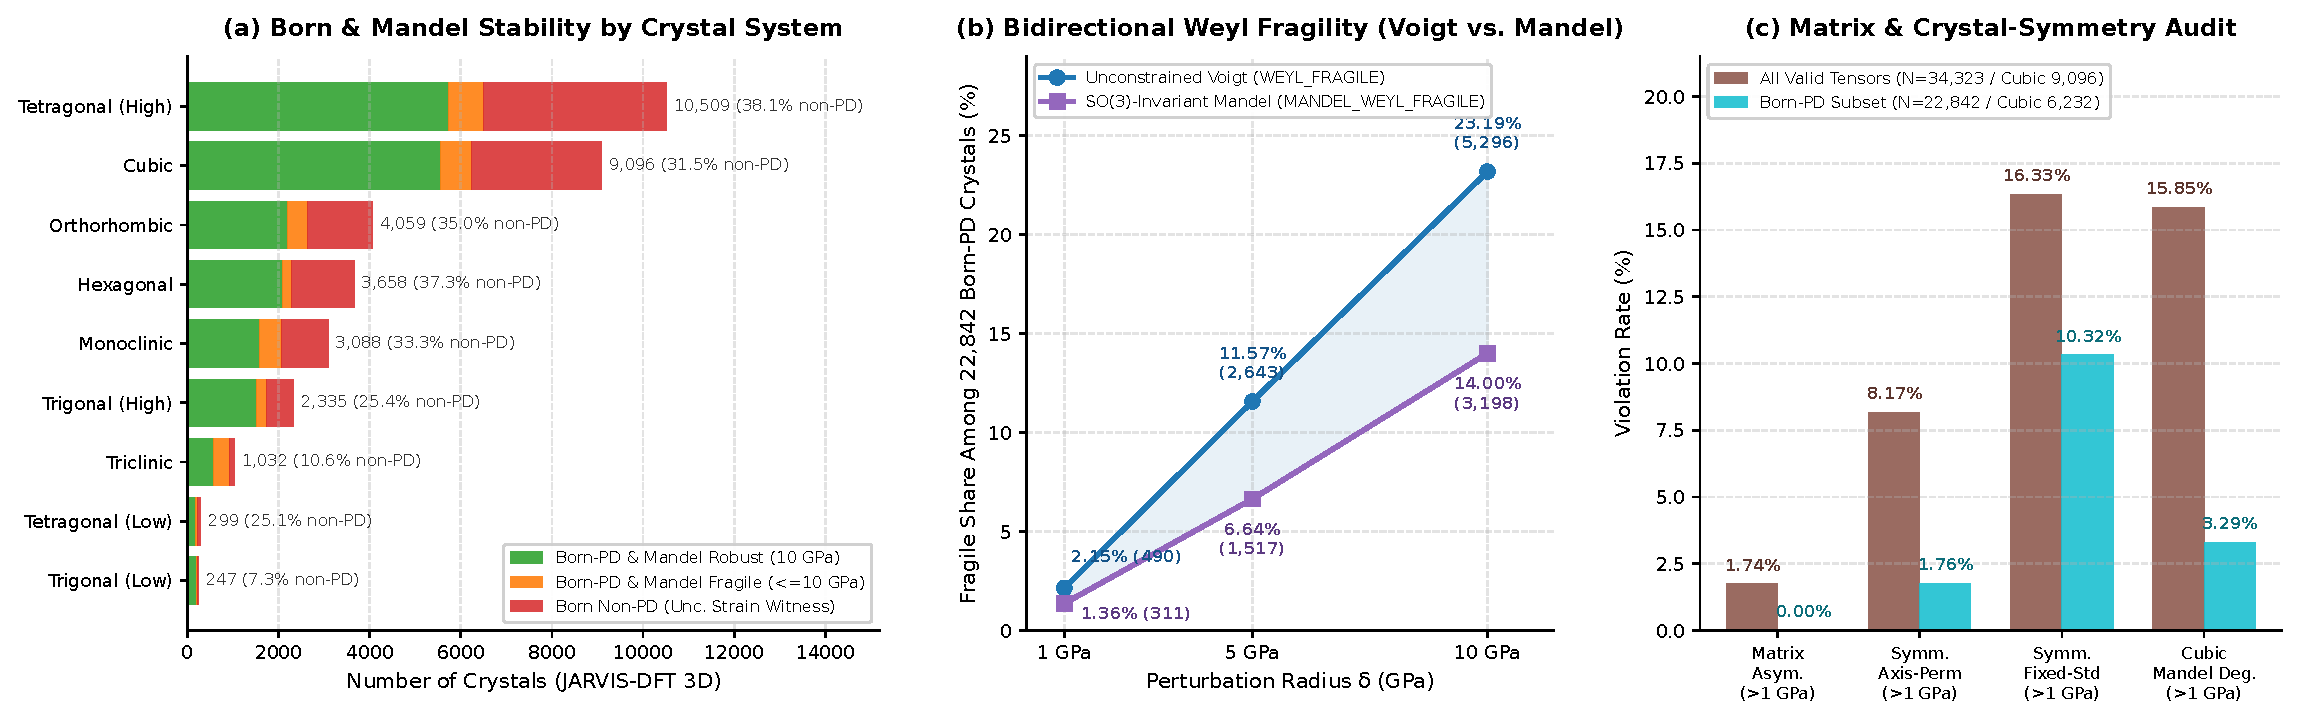
\includegraphics[width=\textwidth]{figures/fig3_jarvis_elastic_born_mandel.pdf}
  \caption{(a) Crystal-system breakdown of 34,323 valid JARVIS elastic tensors into Born non-PD, Born-PD Mandel-fragile, and Born-PD Mandel-robust (10~GPa). (b) Bidirectional Weyl fragility curves across 1/5/10~GPa comparing unconstrained Voigt and $\mathrm{SO}(3)$-invariant Mandel metrics. (c) Matrix asymmetry and crystal-symmetry violation rates across all valid vs.\ Born-PD subsets.}
  \label{fig:elastic}
\end{figure}

\section{Trusted Computing Base, Limitations, and Reproducibility}
All \textbf{95,348} serialized TSV certificates, incremental \texttt{lake build} freshness, \textbf{51/51} \texttt{\#print axioms} checks (0 \texttt{sorryAx}), \textbf{540/540} stratified dataset-binding checks, \textbf{15/15} \texttt{pytest} suites, and the full SHA-256 artifact manifest are verified in one command via \texttt{python reproduce\_all.py {-}{-}verify-only}. Remaining phase evaluations outside the 30,000 serialized phase TSVs are verified in exact Python \texttt{Fraction} arithmetic, intra-catalog GNoME/WBM margins represent upper bounds relative to combined MP+catalog hulls, and \emph{Phase Switching} percentages along exact degenerate ties (e.g., 1,240 zero-margin boundaries in JARVIS) depend on solver tie-breaking.

\paragraph{Code and Data Availability.}
All source code, the standalone Lean~4 verification kernel (\texttt{lean/}), 95,348 machine-verified TSV rational certificates (\texttt{results/}), high-resolution figure generators, and the one-click reproduction suite (\texttt{reproduce\_all.py}) are publicly available under the MIT License at \url{https://github.com/sunpunggi1/certmat} (release \texttt{v1.0.0}). The upstream NIST JARVIS-DFT 3D \texttt{ehull} unit-scaling issue report and minimal reproduction script are filed at \url{https://github.com/usnistgov/jarvis/issues/343}.

\paragraph{Disclosure of AI-Assisted Technologies.}
AI coding and verification agents were used under the author's direction to assist with software engineering, automated database auditing pipelines, and manuscript drafting. All 51 mechanized theorems, 95,348 serialized rational certificates, raw-dataset bindings, and reported empirical metrics are independently verified by the compiled Lean~4 kernel (zero \texttt{sorry}, standard axioms only), an independent pure-\texttt{Fraction} verifier, and deterministic regression tests.

\bibliographystyle{unsrtnat}
\bibliography{references}

\end{document}
